
\section{Cylindrical Projections}
The four cylindrical map projections used for the experimentation are Mercator, Plate Carree, Cylindrical Equal Area, and General Oblique Transformation. The selection of the map projections in done based on the underlying properties of the cylindrical map projections.

\subsection{Mercator}
\begin{figure}[H]
    \centering
    \begin{minipage}{0.30\textwidth}
        \centering
        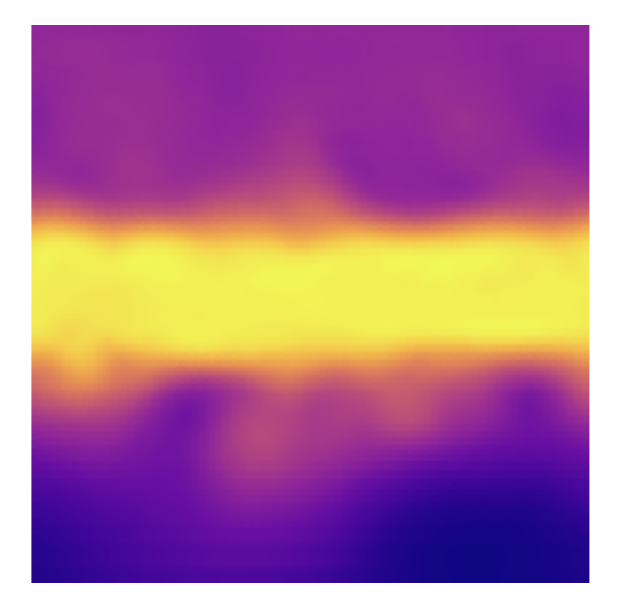
\includegraphics[width=0.9\linewidth]{figures/chapter-8/geopoth_mercator.png}
        \caption{ Geopotential height raster data as Mercator projected}
        \label{fig:merc_geopoth_raster}
    \end{minipage}\hfill
    \begin{minipage}{0.30\textwidth}
        \centering
        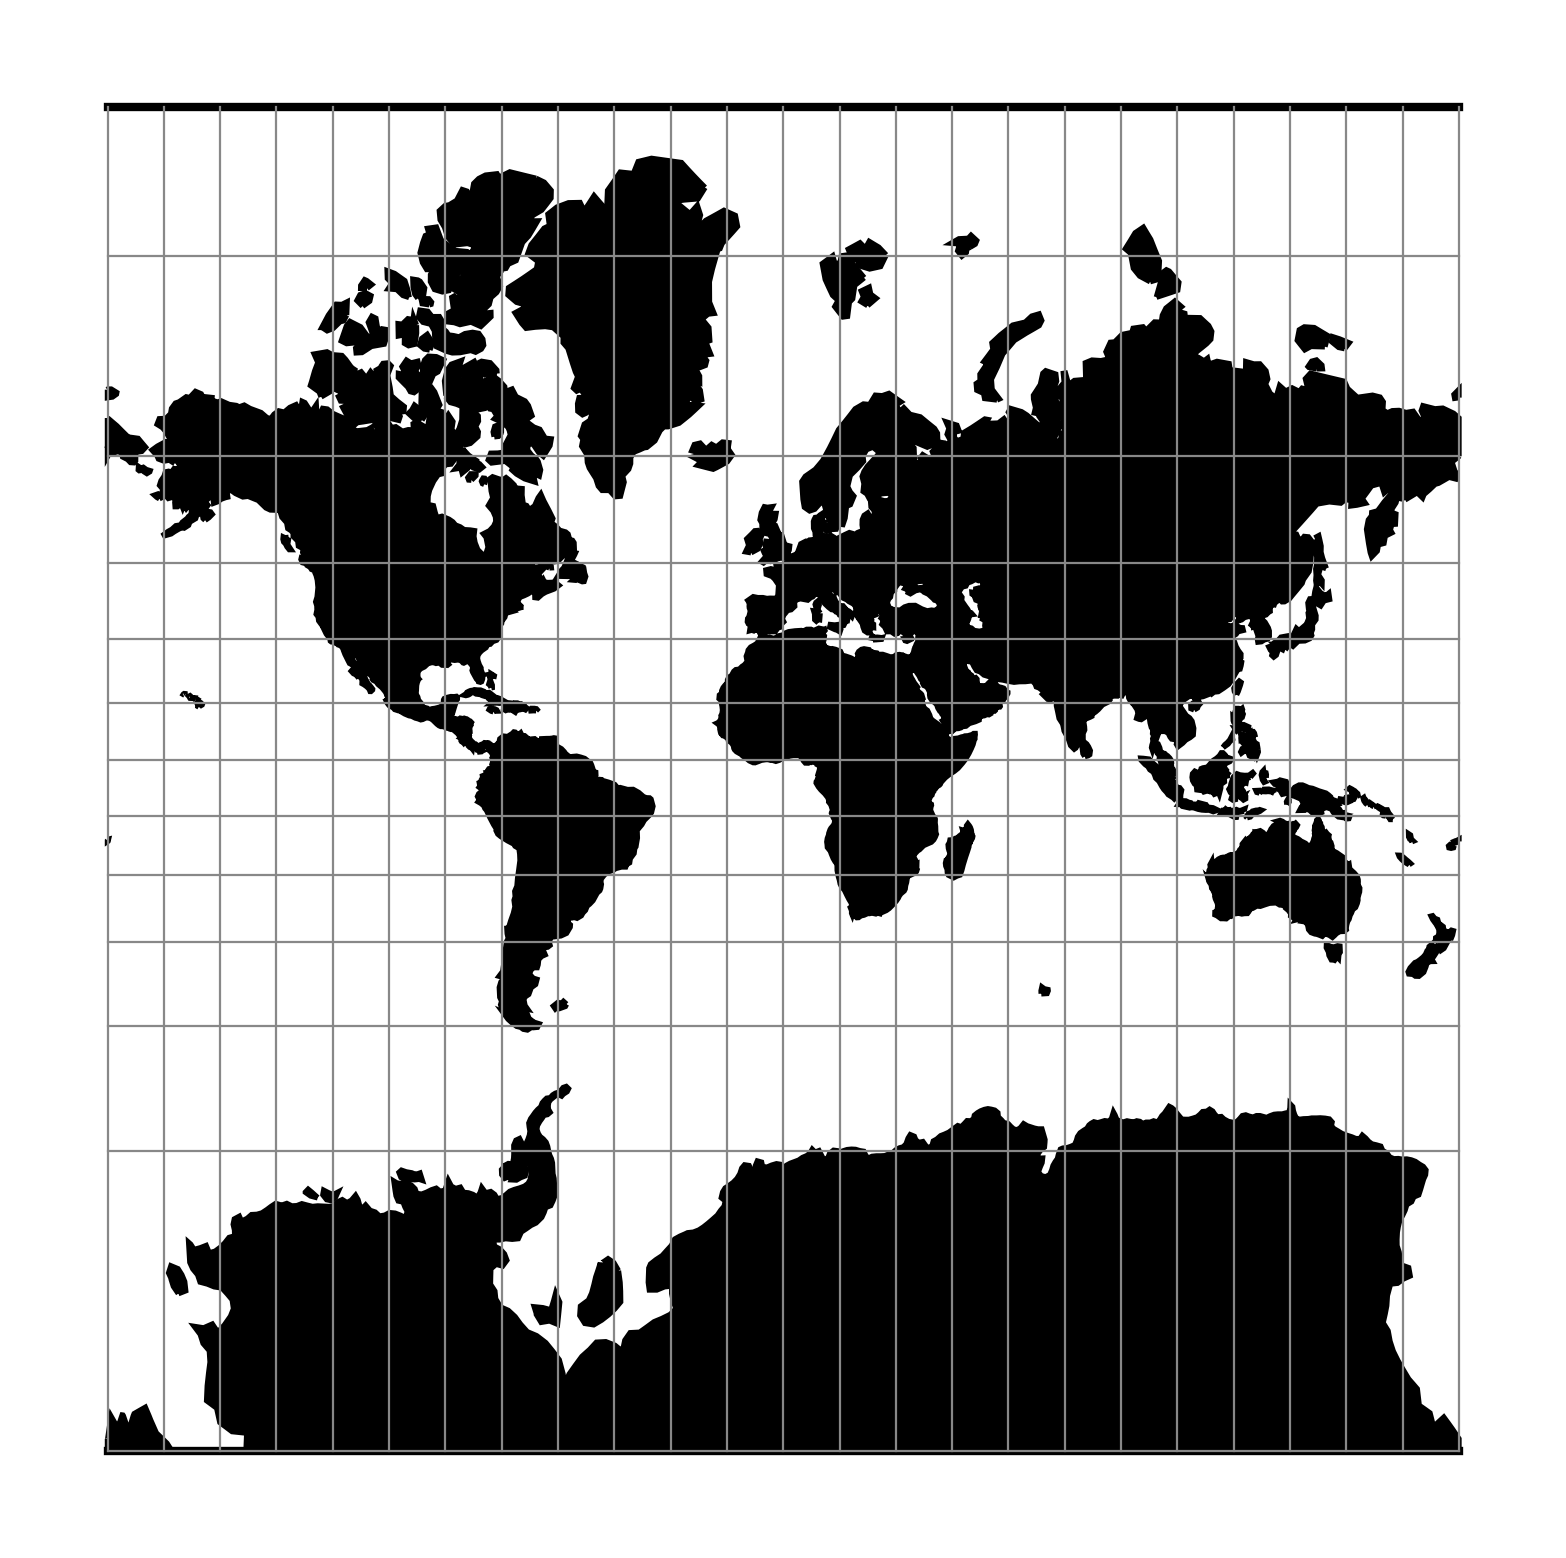
\includegraphics[width=0.9\linewidth]{figures/chapter-8/merc.png}
        \caption{Mercator Projection (Source \cite{PROJ_SITE})}
        \label{fig:merc_proj}
    \end{minipage}\hfill
    \begin{minipage}{0.30\textwidth}
        \centering
        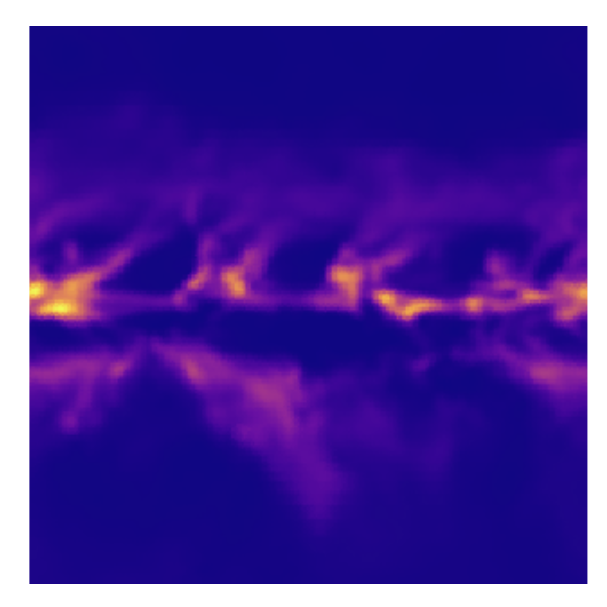
\includegraphics[width=0.9\linewidth]{figures/chapter-8/prect_mercator.png}
        \caption{Precipitation raster data as Mercator projected}
        \label{fig:merc_prect_raster}
    \end{minipage}\hfill
\end{figure}

\begin{figure}[H]
    \centering
    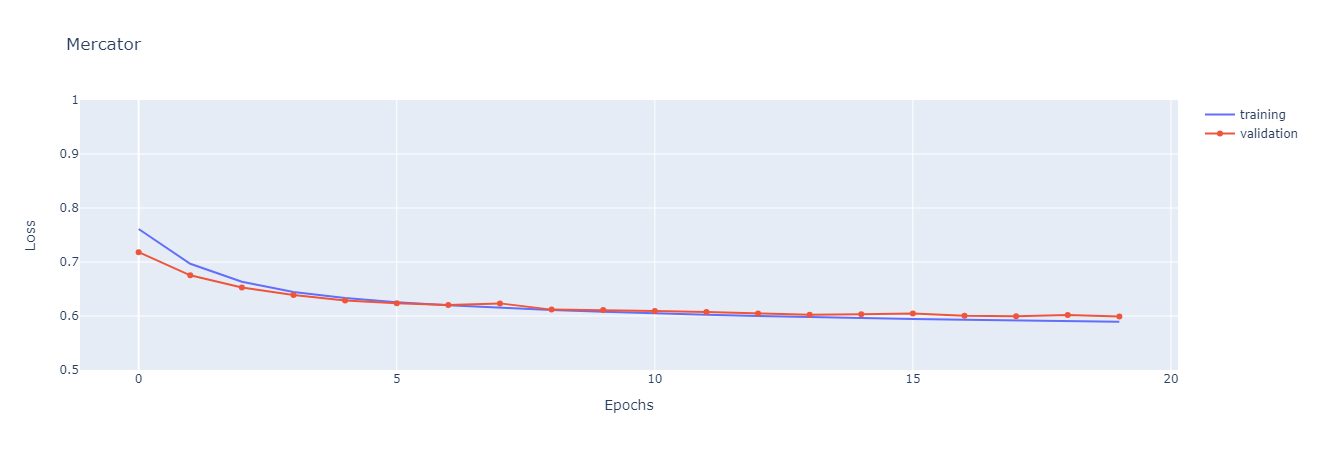
\includegraphics[width=1.0\linewidth]{figures/chapter-8/merc_loss.png}
    \caption{Mercator: Averaged training loss of models  }
    \label{fig:merc_loss}
\end{figure}

\newpage

\subsection{Plate Carree}

\begin{figure}[H]
    \centering
    \begin{minipage}{0.30\textwidth}
        \centering
        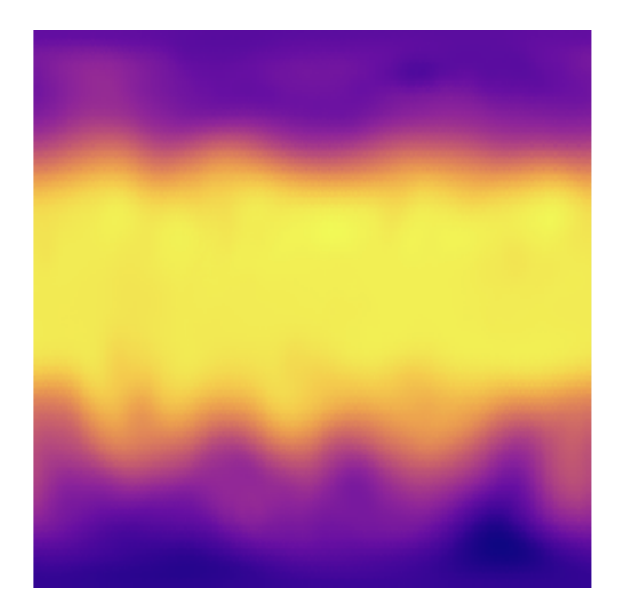
\includegraphics[width=0.9\linewidth]{figures/chapter-8/plate_caree_geopoth_raster.png}
        \caption{ Geopotential height raster data as Plate Carree projected}
        \label{fig:eqc_geopoth_raster}
    \end{minipage}\hfill
    \begin{minipage}{0.30\textwidth}
        \centering
        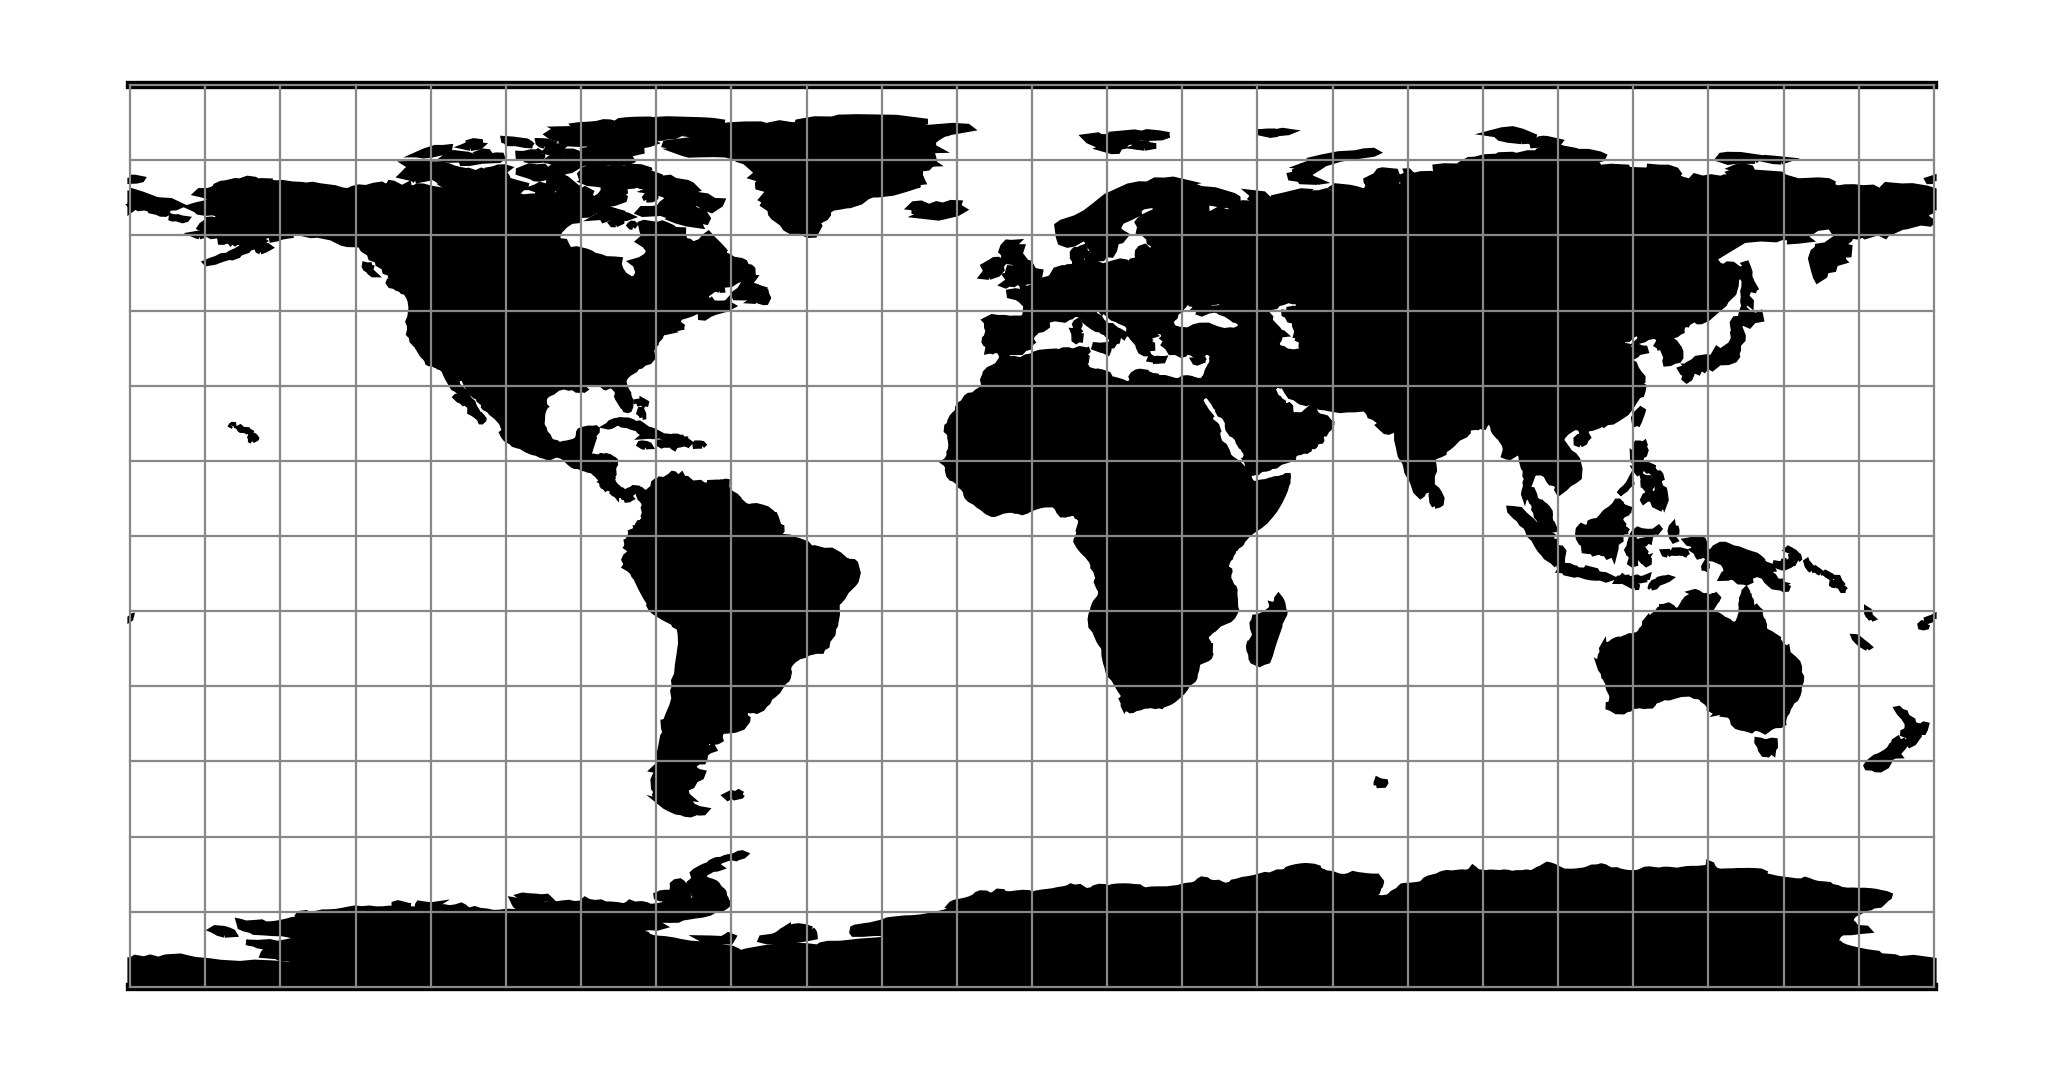
\includegraphics[width=0.9\linewidth]{figures/chapter-8/eqc.png}
        \caption{Plate Carree Projection (Source \cite{PROJ_SITE})}
        \label{fig:eqc_prect_raster}
    \end{minipage}\hfill
    \begin{minipage}{0.30\textwidth}
        \centering
        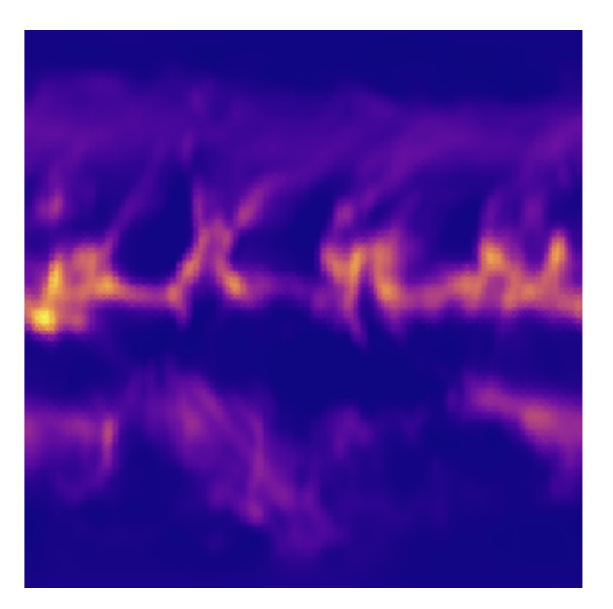
\includegraphics[width=0.9\linewidth]{figures/chapter-8/plate_caree_prect_raster.png}
        \caption{Precipitation raster data as Plate Carree projected}
        \label{fig:eqc_prect_raster}
    \end{minipage}\hfill
\end{figure}

\begin{figure}[H]
    \centering
    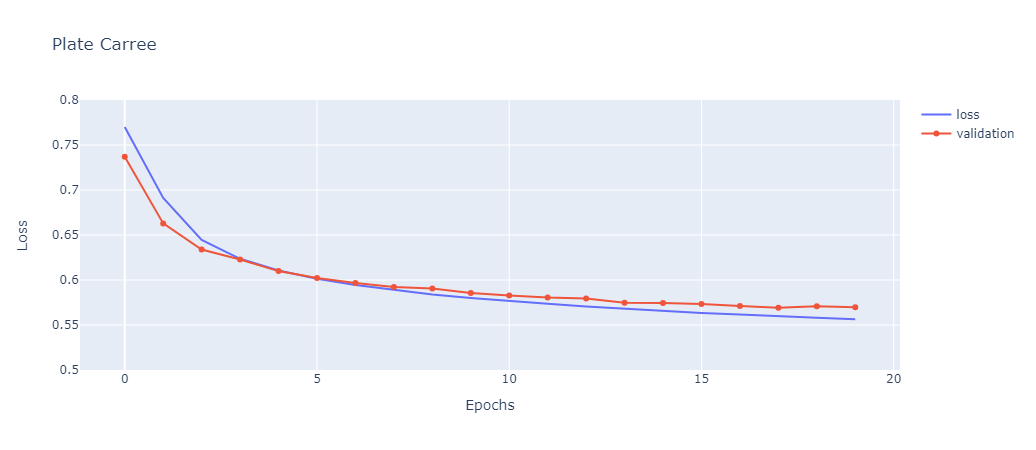
\includegraphics[width=1.0\linewidth]{figures/chapter-8/pc_loss.png}
    \caption{Plate Carree: Averaged training loss of models  }
    \label{fig:pc_loss}
\end{figure}


\subsection{Cylindrical Equal Area}

\begin{figure}[H]
    \centering
    \begin{minipage}{0.30\textwidth}
        \centering
        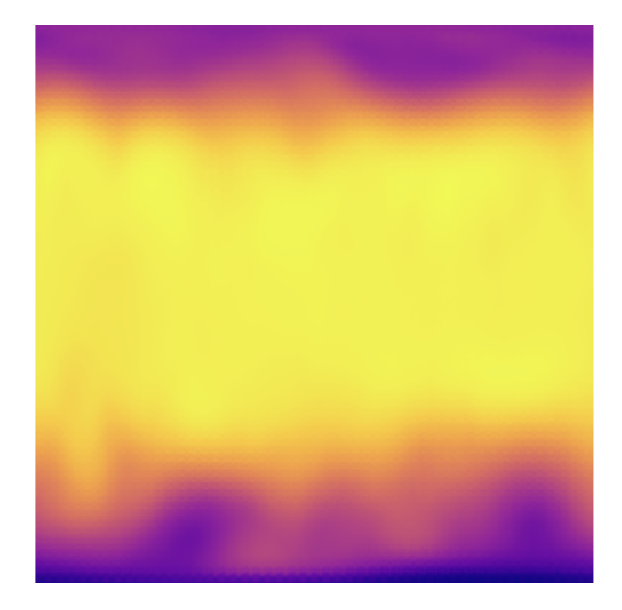
\includegraphics[width=0.9\linewidth]{figures/chapter-8/prect_cea.png}
        \caption{ Geopotential height raster data as Cylindrical Equal Area projected}
        \label{fig:cea_geopoth_raster}
    \end{minipage}\hfill
    \begin{minipage}{0.30\textwidth}
        \centering
        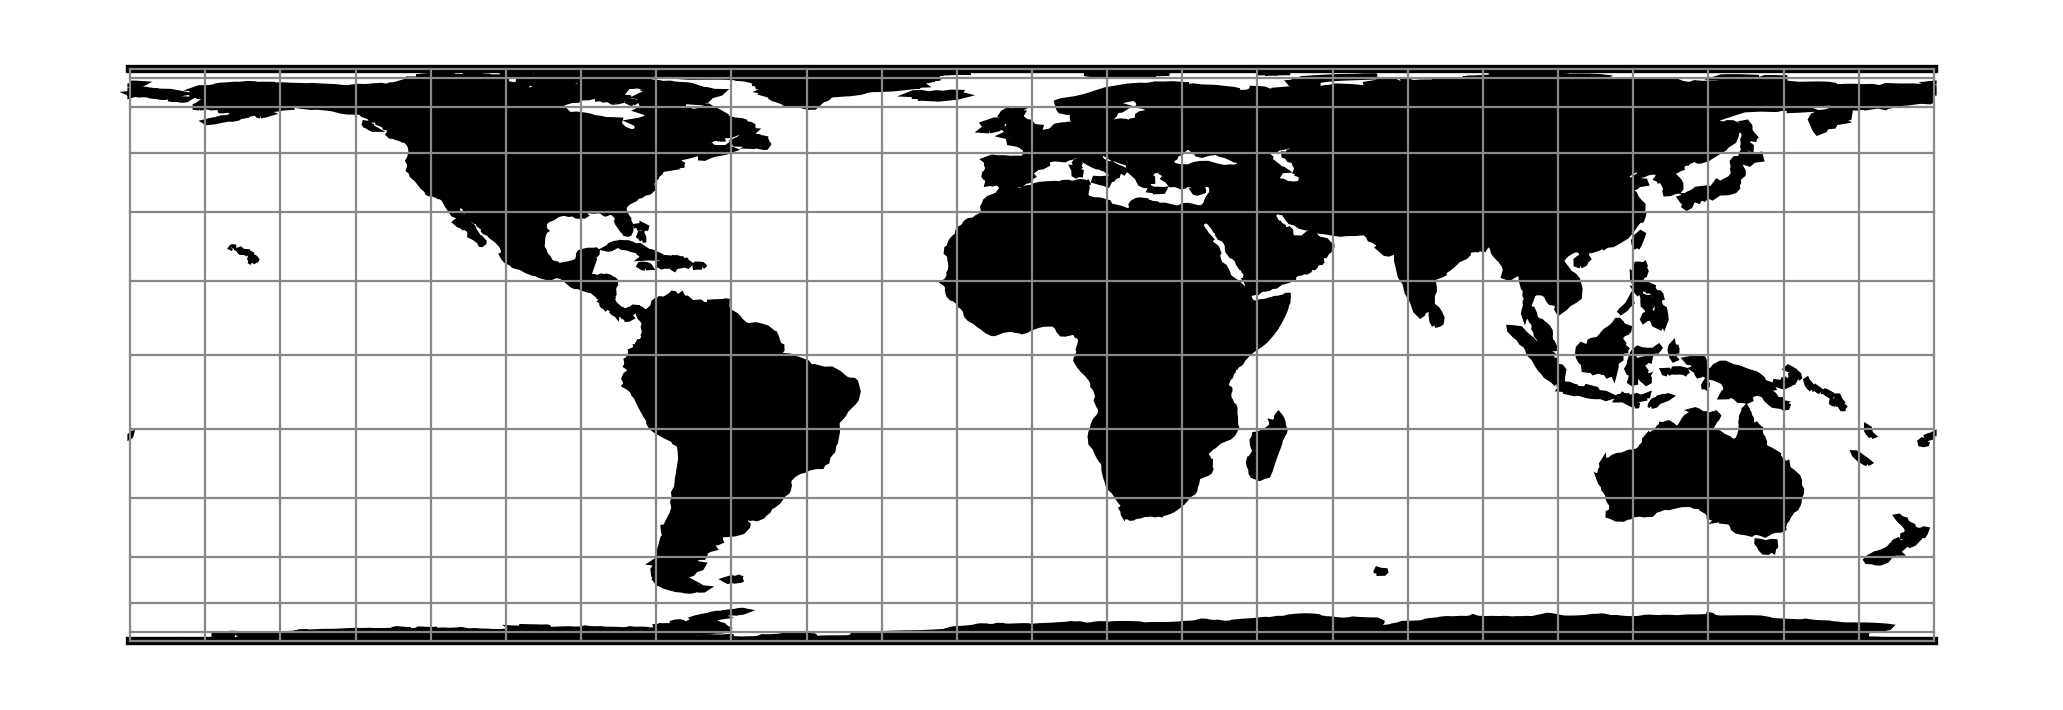
\includegraphics[width=0.9\linewidth]{figures/chapter-8/cea.png}
        \caption{Cylindrical Equal Area Projection (Source \cite{PROJ_SITE})}
        \label{fig:cea_prect_raster}
    \end{minipage}\hfill
    \begin{minipage}{0.30\textwidth}
        \centering
        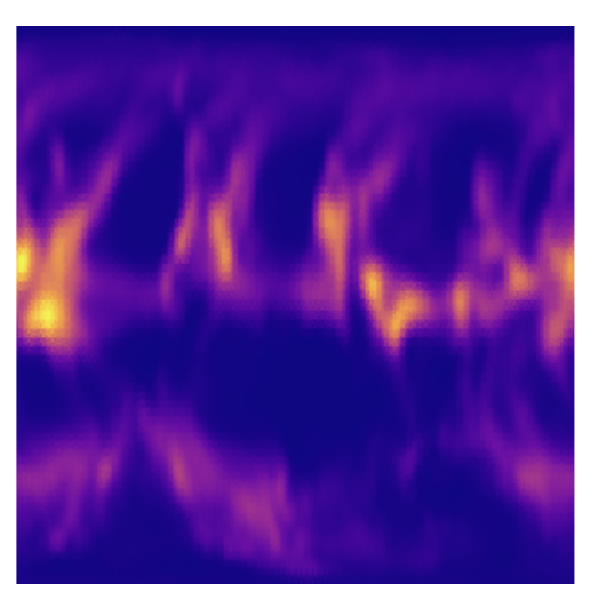
\includegraphics[width=0.9\linewidth]{figures/chapter-8/geopoth_cea.png}
        \caption{Precipitation raster data as Cylindrical Equal Area projected}
        \label{fig:cea_prect_raster}
    \end{minipage}\hfill
\end{figure}

\begin{figure}[h]
    \centering
    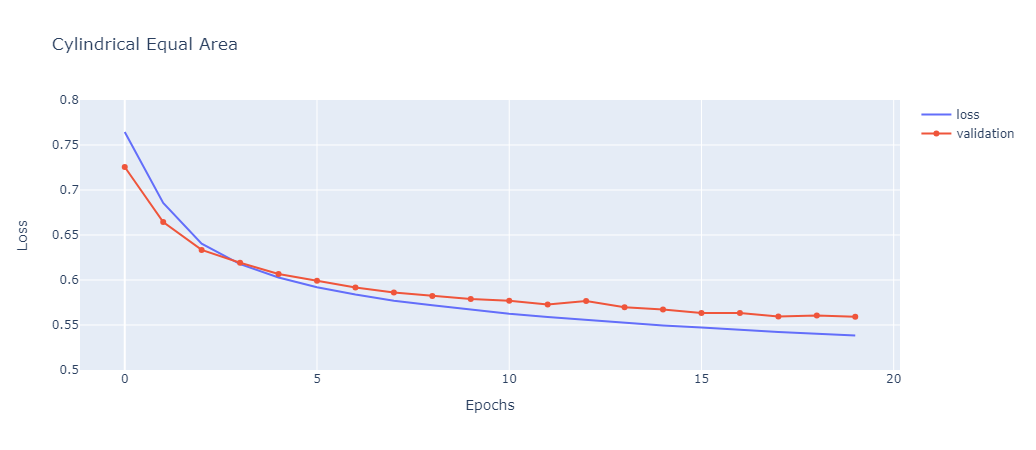
\includegraphics[width=1.0\linewidth]{figures/chapter-8/cea_loss.png}
    \caption{Cylindrical Equal Area: Averaged training loss of models  }
    \label{fig:cea_loss}
\end{figure}

\subsection{General Oblique Transformation}
\begin{figure}[H]
    \centering
    \begin{minipage}{0.30\textwidth}
        \centering
        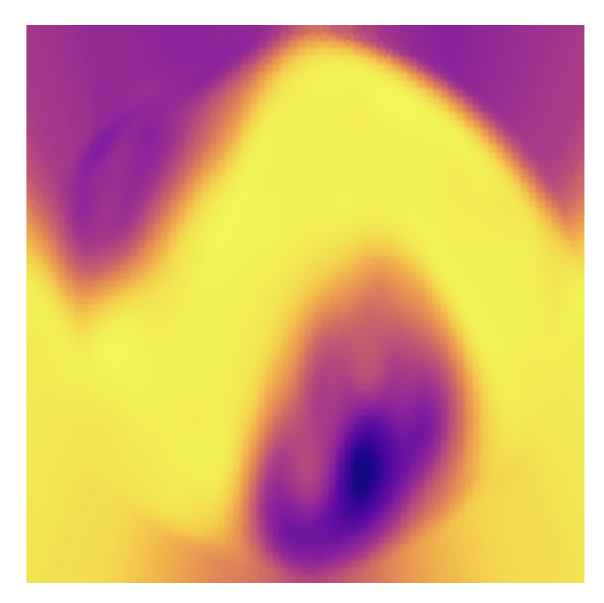
\includegraphics[width=0.9\linewidth]{figures/chapter-8/geopoth_got.png}
        \caption{ Geopotential height raster data as General Oblique Transformation projected}
        \label{fig:ob_tran_geopoth_raster}
    \end{minipage}\hfill
    \begin{minipage}{0.30\textwidth}
        \centering
        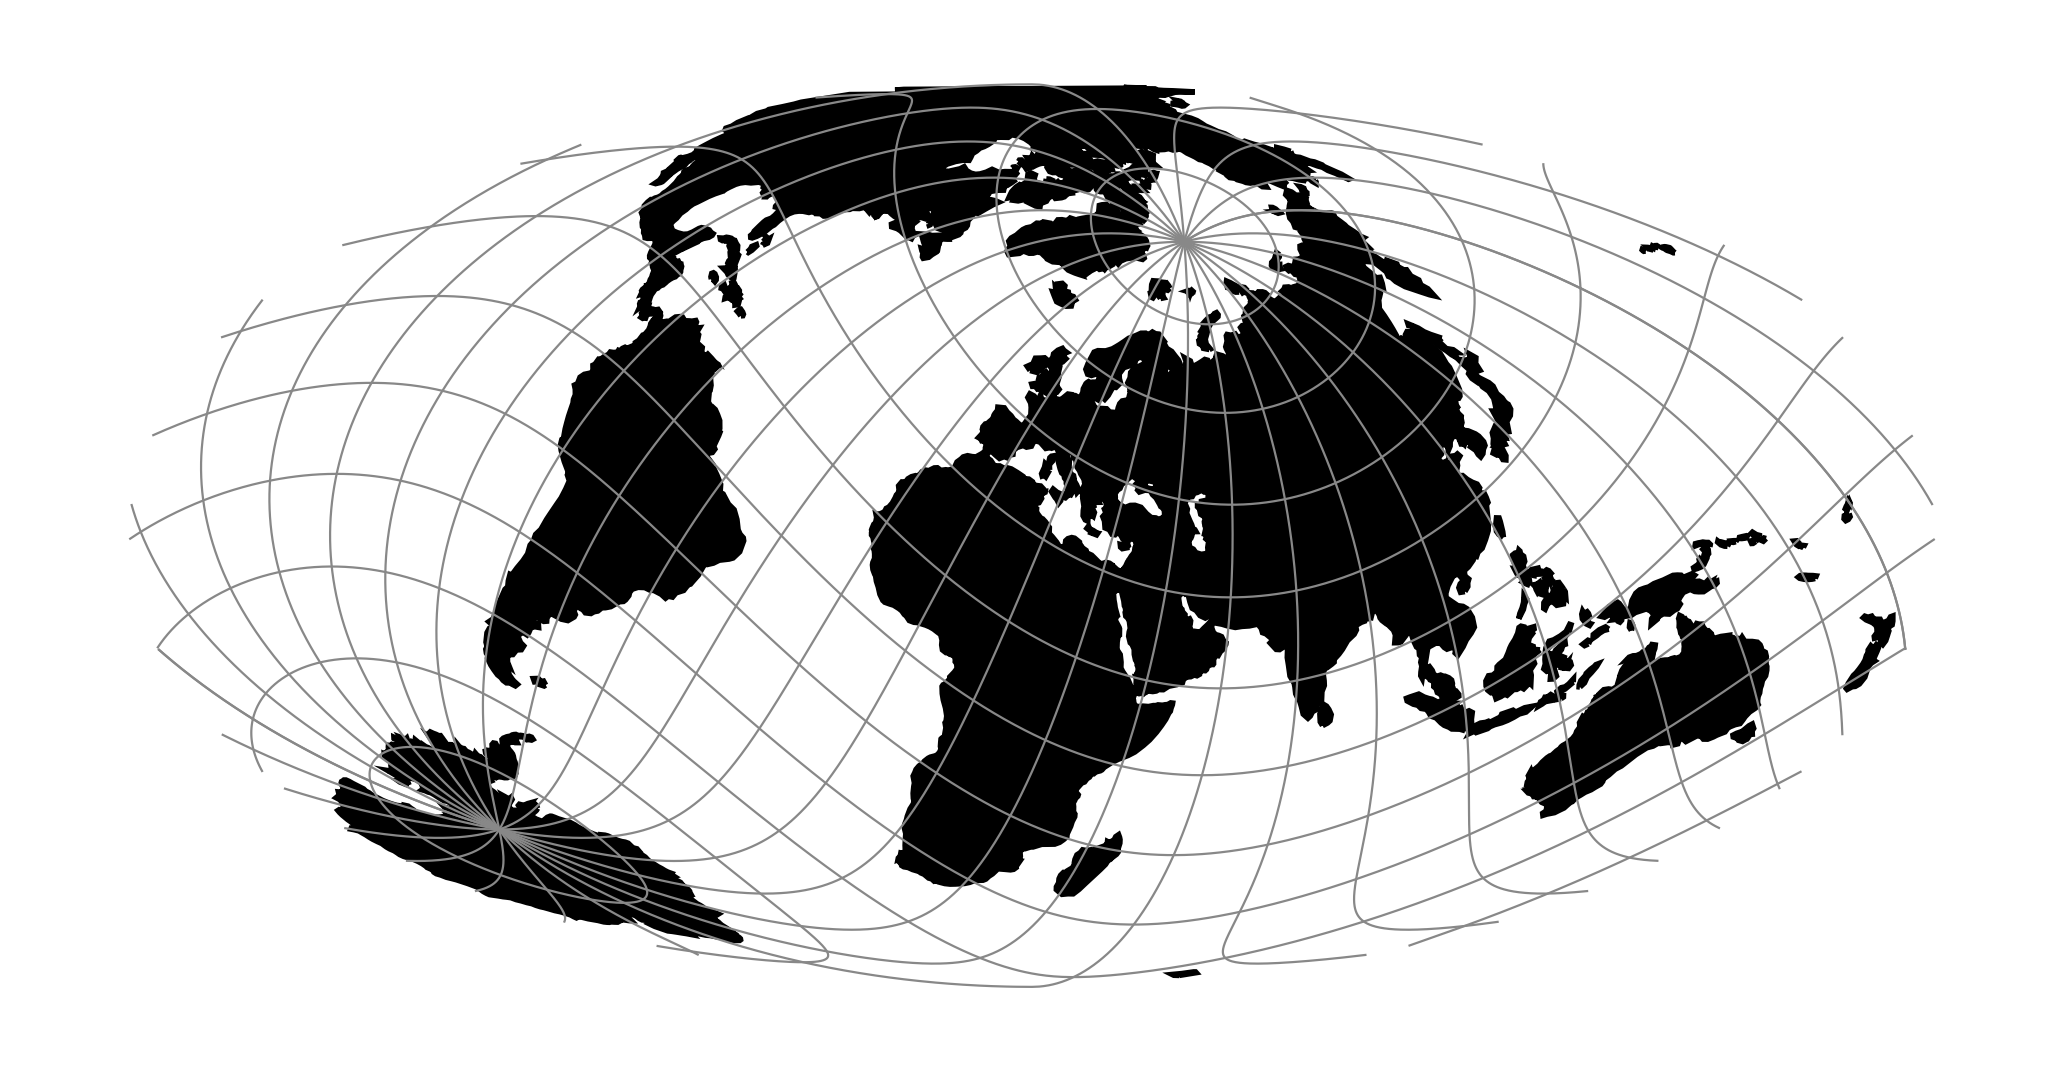
\includegraphics[width=0.9\linewidth]{figures/chapter-8/ob_tran.png}
        \caption{General Oblique Transformation Projection (Source \cite{PROJ_SITE})}
        \label{fig:ob_tran_proj}
    \end{minipage}\hfill
    \begin{minipage}{0.30\textwidth}
        \centering
        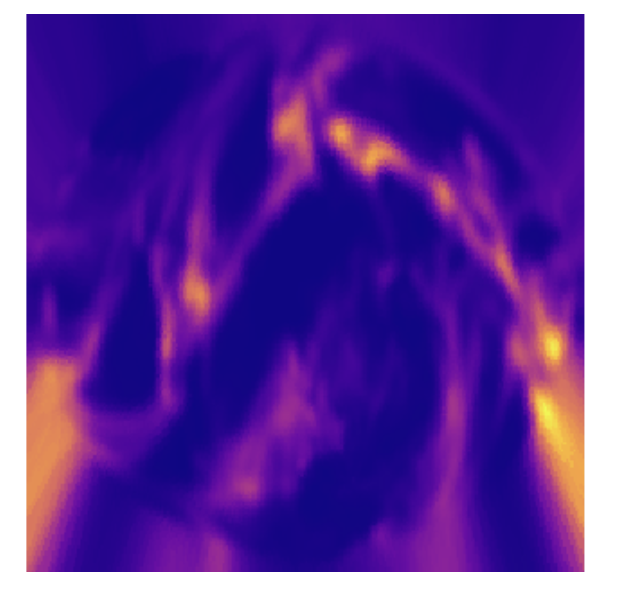
\includegraphics[width=0.9\linewidth]{figures/chapter-8/prect_got.png}
        \caption{Precipitation raster data as General Oblique Transformation projected}
        \label{fig:ob_tran_prect_raster}
    \end{minipage}\hfill
\end{figure}

\begin{figure}[H]
    \centering
    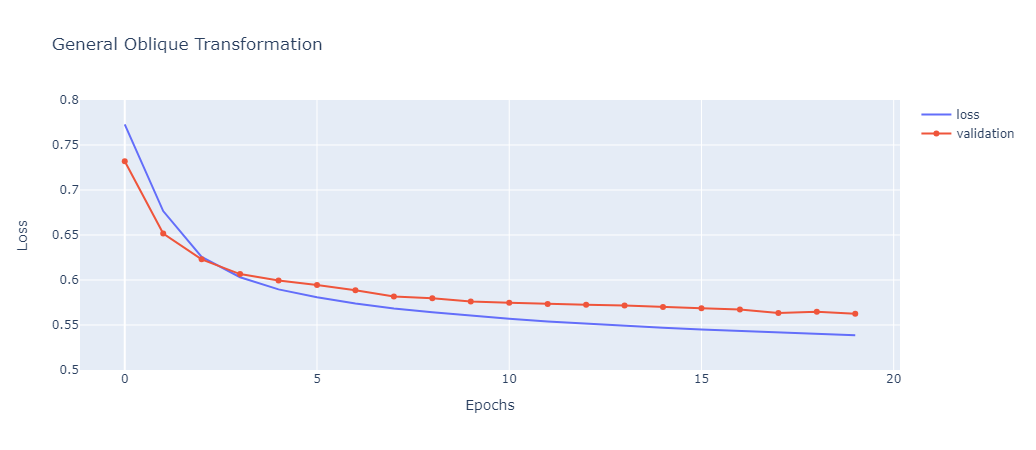
\includegraphics[width=1.0\linewidth]{figures/chapter-8/got_loss.png}
    \caption{General Oblique Transformation: Averaged training loss of models  }
    \label{fig:got_loss}
\end{figure}
\subsection{Results}
\begin{table}[ht]
    \centering
    \caption{Summary of Model Performance}
    \label{cylindrical_results_table}
    \renewcommand{\arraystretch}{1.2} % Adjusts the row height
    \begin{tabular}{|l|c|c|c|c|c|}
        \hline
        \rowcolor[gray]{0.9}
        \textbf{\emph{Project Name}} & \textbf{\emph{\# Epochs}} & \textbf{\emph{MAE}} & \textbf{\emph{Validation MAE}} & \textbf{\emph{MAPE}} & \textbf{\emph{Validation MAPE}} \\ \hline
        Project 1                    & 50                        & 0.05                & 0.06                           & 5\%                  & 6\%                             \\ \hline
        Project 2                    & 30                        & 0.04                & 0.05                           & 4\%                  & 5\%                             \\ \hline
        Project 3                    & 100                       & 0.03                & 0.04                           & 3\%                  & 4\%                             \\ \hline
    \end{tabular}
\end{table}